\documentclass[12pt,letterpaper,twoside]{article}
\usepackage{amsmath,amssymb,amsfonts}
\usepackage{graphicx}
\usepackage{tikz}
\usepackage{pgfplots}
\pgfplotsset{compat=1.17}
\usepackage{xcolor}
\usepackage{hyperref}
\usepackage{cleveref}
\usepackage{booktabs}
\usepackage{caption}
\usepackage{subcaption}
\usepackage{wrapfig}
\usepackage{nicefrac}
\usepackage{minted}
\usepackage{geometry}
\geometry{margin=1in, top=0.75in, bottom=0.75in}

% Colors for physicality of confusion
\definecolor{phyblue}{RGB}{31, 119, 180}
\definecolor{phygreen}{RGB}{44, 160, 44}
\definecolor{phyred}{RGB}{214, 39, 40}
\definecolor{phypurple}{RGB}{148, 103, 189}
\definecolor{phyorange}{RGB}{255, 127, 14}
\definecolor{phyteal}{RGB}{44, 174, 175}
\definecolor{phyyellow}{RGB}{188, 189, 34}

% TikZ libraries
\usetikzlibrary{decorations.pathmorphing,shapes.geometric,calc,positioning,arrows.meta,patterns,3d}

% Title and Author
\title{\textbf{The Physicality of Confusion: Energy-Modulated Metrics and Reactive Plasticity in Finslerian Neural Networks}}

\author{Joaquin Stürtz}

\date{January 26, 2026}

% Header
\pagestyle{myheadings}
\markright{The Physicality of Confusion}
\lhead{Manifold Learning Research}
\rhead{\thepage}

% Theorem-like environments
\newtheorem{definition}{Definition}[section]
\newtheorem{theorem}{Theorem}[section]
\newtheorem{Lemma}{Lemma}[section]
\newtheorem{example}{Example}[section]
\newtheorem{remarque}{Remark}[section]
\newtheorem{prop}{Proposition}[section]
\newtheorem{corol}{Corollary}[section]

% Macros for frequently used notation
\newcommand{\M}{\mathcal{M}}
\newcommand{\R}{\mathbb{R}}
\newcommand{\T}{\mathbb{T}}
\newcommand{\Sph}{\mathbb{S}}
\newcommand{\diff}{\mathrm{d}}
\DeclareMathOperator{\diag}{diag}
\DeclareMathOperator{\sech}{sech}

\begin{document}

\maketitle
\thispagestyle{empty}

\vspace{0.5cm}

\begin{abstract}
Standard Riemannian Manifold Learning assumes a metric $g(x)$ that is independent of the state velocity, implying a static geometry for the latent space. We introduce \textbf{Reactive Plasticity}, a framework where the manifold geometry deforms dynamically based on the \textbf{Kinetic Energy} of the neural state. By mapping semantic ``Confusion''---manifested as high-velocity oscillations---to the elasticity of the geometric connection, we create a self-regulatory inductive bias. This formulation transitions the latent space into a \textbf{Finsler Manifold}, where the local speed limit of reasoning is governed by the model's instantaneous certainty. We further explore the emergence of \textbf{Semantic Singularities}, where extreme confidence or ambiguity creates ``black holes'' in the manifold that trap or repel trajectories. This coupling provides a deterministic uncertainty proxy and an internal stabilization mechanism that generalizes gradient clipping to an intrinsic geometric property.
\end{abstract}

\vspace{0.5cm}
\hrule
\vspace{0.5cm}

\tableofcontents
\newpage

\section{Beyond Static Riemannian Metrics}

In conventional deep learning architectures, the distance between semantic concepts is fixed by the static parameters of the network. Even in manifold-based approaches, the metric $g(x)$ typically depends only on the position $x$ in the latent space. This assumes that the ``difficulty'' of traversing a semantic region is independent of how fast the model is attempting to process information.

\begin{prop}[Static Metric Assumption]
Standard Riemannian geometry assumes:
\[
g: \M \to \text{Symmetric}(d, \mathbb{R}), \quad x \mapsto g(x),
\]
where the metric depends only on position, not on the direction or speed of traversal.
\end{prop}

However, in biological and physical systems, high-speed transitions often involve dissipation, friction, or changes in material properties:

\begin{remarque}[Physical Systems]
\begin{itemize}
\item \textbf{Biological muscles}: Stiffen during rapid movements to prevent injury.
\item \textbf{Non-Newtonian fluids}: Increase viscosity under shear stress (shear-thickening).
\end{itemize}
\end{remarque}

We argue that ``Confusion'' in a neural network is not merely a statistical state but a physical property of the manifold's dynamics:

\begin{prop}[Confusion as Physical Property]
When a model encounters ambiguous or contradictory input:
\begin{enumerate}
\item The latent state undergoes rapid, high-energy fluctuations.
\end{enumerate}
By making the geometry reactive to this energy, we enforce stability and provide a natural measure of uncertainty.
\end{prop}

\begin{figure}[htbp]
centering
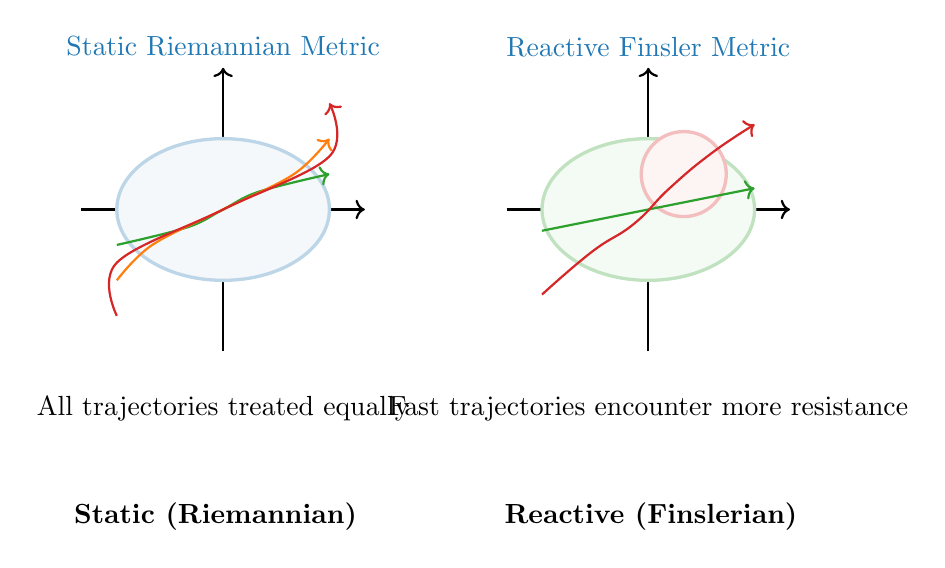
\begin{tikzpicture}[scale=0.9]
    % Static vs Reactive geometry
    \begin{scope}[shift={(0, 0)}]
        % Static geometry (left)
        \draw[->, thick] (-2, 0) -- (2, 0);
        \draw[->, thick] (0, -2) -- (0, 2);
        
        \draw[phyblue!30, fill=phyblue!5, very thick] ellipse (1.5 and 1);
        \node[phyblue] at (0, 2.3) {Static Riemannian Metric};
        
        % Trajectories at different speeds
        \foreach \v/\col in {0.5/phygreen, 1.0/phyorange, 1.5/phyred} {
            \draw[\col, thick, ->] 
                plot[smooth,tension=0.6] coordinates {
                    (-1.5, -\v) (-\v, -\v/2) (0, 0) (\v, \v/2) (1.5, \v)
                };
        }
        
        \node[below] at (0, -2.5) {All trajectories treated equally};
    \end{scope}
    
    % Reactive geometry (right)
    \begin{scope}[shift={(6, 0)}]
        \draw[->, thick] (-2, 0) -- (2, 0);
        \draw[->, thick] (0, -2) -- (0, 2);
        
        % Variable geometry - low energy region
        \draw[phygreen!30, fill=phygreen!5, very thick] ellipse (1.5 and 1);
        
        % Variable geometry - high energy region (curved)
        \draw[phyred!30, fill=phyred!5, very thick] 
            (0.5, 0.5) circle (0.6);
            
        \node[phyblue] at (0, 2.3) {Reactive Finsler Metric};
        
        % Slow trajectory (easy path)
        \draw[phygreen, thick, ->] 
            plot[smooth,tension=0.6] coordinates {
                (-1.5, -0.3) (-0.5, -0.1) (0.5, 0.1) (1.5, 0.3)
            };
            
        % Fast trajectory (curved path)
        \draw[phyred, thick, ->] 
            plot[smooth,tension=0.8] coordinates {
                (-1.5, -1.2) (-0.8, -0.6) (-0.2, -0.2) (0.3, 0.3) (0.9, 0.8) (1.5, 1.2)
            };
            
        \node[below] at (0, -2.5) {Fast trajectories encounter more resistance};
    \end{scope}
    
    % Labels
    \node[below] at (3, -4) {\textbf{Static (Riemannian)} \quad\quad\quad\quad\quad \textbf{Reactive (Finslerian)}};
\end{tikzpicture}
caption{Static versus reactive geometry. Left: All trajectories are treated equally regardless of speed. Right: Fast trajectories (high energy/``confusion'') encounter increased curvature, acting as a geometric brake.}
\labelfig:static-vs-reactive}
\end{figure}

This transitions the latent space into a Finsler Manifold, where the local speed limit of reasoning is governed by the model's instantaneous certainty.

\section{The Finslerian Formalism in Latent Space}

To model velocity-dependent geometry, we move from Riemannian geometry to Finsler Geometry.

\begin{definition}[Finsler Manifold]
A Finsler manifold is characterized by a Minkowski norm $F(x, v)$ on each tangent space, leading to a metric tensor $g_{ij}(x, v)$ that depends on both position $x$ and velocity $v$.
\end{definition}

This is the key distinction from Riemannian geometry: the metric now carries information about how the model is traversing the latent space, not just where it is.

\begin{remarque}[Finsler vs. Riemannian]
\begin{itemize}
\item \textbf{Riemannian}: $g = g(x)$, static geometry.
\item \textbf{Finslerian}: $g = g(x, v)$, dynamic geometry that adapts to traversal speed.
\end{itemize}
\end{remarque}

\begin{prop}[Key Advantage]
The Finslerian formulation allows the manifold to ``know'' how fast the state is moving and adjust its resistance accordingly---modeling the physical intuition that rapid transitions require more caution.
\end{prop}

\begin{figure}[htbp]
centering
\begin{tikzpicture}[scale=0.85]
    % Unit ball comparison
    \begin{scope}[x={(0.8cm,0.2cm)},y={(-0.3cm,0.7cm)},z={(0,0.8cm)}]
        % Riemannian unit ball (Euclidean)
        \draw[phyblue, thick, fill=phyblue!10] 
            plot[domain=0:360, variable=\t, samples=60] 
            ({cos(\t)}, {sin(\t)}, {0});
            
        % Finslerian unit ball (asymmetric)
        \draw[phyred, thick, fill=phyred!10, dashed] 
            plot[domain=0:360, variable=\t, samples=60] 
            ({0.6*cos(\t) + 0.3*sin(2*\t)}, {0.6*sin(\t) + 0.3*cos(2*\t)}, {0});
            
        % Velocity-dependent expansion
        \foreach \v in {0.5, 1.0, 1.5} {
            \draw[phypurple!\v*60, thick] 
                plot[domain=0:360, variable=\t, samples=30] 
                ({(0.8+0.1*\v)*cos(\t)}, {(0.8+0.1*\v)*sin(\t)}, {0});
        }
        
        % Labels
        \node[phyblue, below] at (0, -1.2, 0) {Riemannian $B_1(0)$};
        \node[phyred, below] at (1.2, -1.2, 0) {Finsler $B_1(0, v)$};
    \end{scope}
    
    % Legend
    \node[right] at (5, 1) {\textbf{Finsler Metric Properties}};
    \node[right] at (5, 0.5) {$F(x, v) = \sqrt{g_{ij}(x,v)v^i v^j}$};
    \node[right] at (5, 0) {$g_{ij}(x,v)$ depends on velocity};
    \node[right] at (5, -0.5) {Asymmetric unit ball};
    \node[right] at (5, -1) {Non-reversible geodesics};
\end{tikzpicture}
caption{Riemannian versus Finslerian unit balls. The Finslerian unit ball (red dashed) is asymmetric and velocity-dependent, reflecting the direction-dependent geometry of reactive plasticity.}
\labelfig:finsler-geometry}
\end{figure}

\subsection{The Plasticity Scalar}

We define the \textbf{Plasticity Scalar} $\Phi(x, v)$ as a measure of the semantic ``temperature'' or kinetic energy:

\begin{definition}[Plasticity Scalar]
\[
\Phi(x, v) = \lambda \cdot \tanh\left(\frac{1}{d} \sum_{i=1}^d v_i^2\right),
\]
where $\lambda$ is the \textbf{Plasticity Coefficient} determining maximum geometric deformation.
\end{definition}

The hyperbolic tangent ensures:
\begin{enumerate}
\item \textbf{Bounded response}: $\Phi \in [0, \lambda]$.
\end{enumerate}

This prevents numerical instability while allowing nonlinear response to energy spikes.

\begin{remarque}[Physical Interpretation]
The plasticity scalar models the material's response to stress:
\begin{itemize}
\item Low stress (low energy): Minimal deformation.
\item High stress (high energy): Maximum deformation (yield point).
\end{itemize}
\end{remarque}

\begin{prop}[Kinetic Energy Relation]
The argument of tanh is proportional to the kinetic energy:
\[
K = \frac{1}{2}\|v\|^2 = \frac{1}{2}\sum_{i=1}^d v_i^2.
\]
Thus $\Phi$ increases with the energy of the neural state.
\end{prop}

\begin{figure}[htbp]
centering
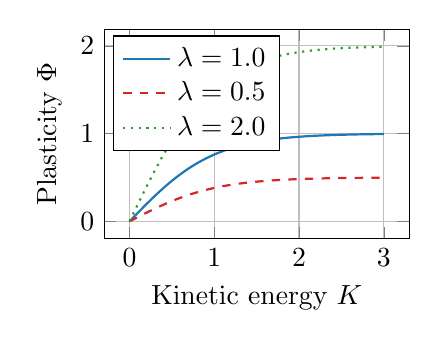
\begin{tikzpicture}
\begin{axis}[
    width=0.45\textwidth,
    height=0.35\textwidth,
    xlabel={Kinetic energy $K$},
    ylabel={Plasticity $\Phi$},
    grid=major,
    samples=100,
    domain=0:3,
    legend pos=north west
]
\addplot[phyblue, thick] {tanh(x)};
\addlegendentry{$\lambda = 1.0$}

\addplot[phyred, dashed, thick] {0.5 * tanh(x)};
\addlegendentry{$\lambda = 0.5$}

\addplot[phygreen, dotted, thick] {2.0 * tanh(x)};
\addlegendentry{$\lambda = 2.0$}
\end{axis}
\end{tikzpicture}
\hfill
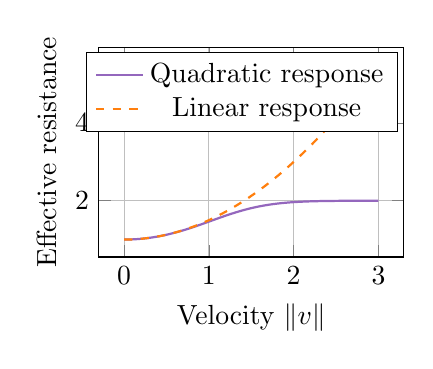
\begin{tikzpicture}
\begin{axis}[
    width=0.45\textwidth,
    height=0.35\textwidth,
    xlabel={Velocity $\|v\|$},
    ylabel={Effective resistance},
    grid=major,
    samples=100,
    domain=0:3,
]
\addplot[phypurple, thick] {1 + tanh(x*x/2)};
\addlegendentry{Quadratic response}

\addplot[phyorange, dashed, thick] {1 + 0.5 * x*x};
\addlegendentry{Linear response}
\end{axis}
\end{tikzpicture}
\textbf{Left:} Plasticity scalar as a function of kinetic energy. \textbf{Right:} Effective resistance to motion increases with velocity.}
\labelfig:plasticity-response}
\end{figure}

\subsection{Reactive Curvature Dynamics}

The effective connection governing geodesic flow is modulated by plasticity:

\begin{definition}[Reactive Connection]
\[
\Gamma_{\text{eff}}^k{}_{ij}(x, v) = \Gamma_{\text{static}}^k{}_{ij}(x) \cdot \left(1 + \Phi(x, v)\right).
\]
\end{definition}

This modulation has profound implications for the dynamics:

\begin{prop}[Flow Regimes]
\begin{enumerate}
\item \textbf{Laminar Flow} ($v \to 0$): $\Phi \approx 0$. The geometry is governed by the static metric, allowing efficient low-resistance transitions.
\item \textbf{Turbulent Flow} (High $v$): $\Phi$ grows. Christoffel symbols increase, acting as geometric brakes that resist acceleration.
\end{enumerate}
\end{prop}

\begin{remarque}[Physical Analogy]
The reactive connection behaves like a variable-resistance medium:
\begin{itemize}
\item \textbf{Laminar regime}: Low viscosity, easy flow.
\item \textbf{Turbulent regime}: High viscosity, resistance to rapid motion.
\end{itemize}
\end{remarque}

\begin{figure}[htbp]
centering
\begin{tikzpicture}[scale=0.9]
    % Flow visualization
    \begin{scope}[x={(0.7cm,0.2cm)},y={(-0.3cm,0.6cm)},z={(0,0.8cm)}]
        % Streamlines at different speeds
        \foreach \v/\col/\lab in {0.3/phygreen/slow, 0.7/phypurple/medium, 1.2/phyred/fast} {
            \draw[\col, thick, ->] 
                plot[smooth,tension=0.5] coordinates {
                    (-2, -\v, 0) (-1, -\v*0.6) (0, 0) (1, \v*0.6) (2, \v, 0)
                };
        }
        
        % Curvature field (increasing with y)
        \foreach \y in {-1.5, -0.5, 0.5, 1.5} {
            \foreach \x in {-1.5, -0.5, 0.5, 1.5} {
                \draw[\phyblue!\numexpr50+\y*30, thick, rotate=\y*20] 
                    (\x, \y, 0) circle (0.1 + 0.05*\y);
            }
        }
        
        % Labels
        \node[phygreen, below left] at (-2, -0.5, 0) {Laminar};
        \node[phyred, above right] at (2, 1.5, 0) {Turbulent};
    \end{scope}
    
    % Regime description
    \node[right] at (5, 1) {\textbf{Flow Regimes}};
    \node[right] at (5, 0.5) {$\Phi \approx 0$: Efficient traversal};
    \node[right] at (5, 0) {$\Phi > 0$: Increased resistance};
    \node[right] at (5, -0.5) {$\Phi \gg 0$: Geometric braking};
    \node[right] at (5, -1) {Self-regulatory stability};
\end{tikzpicture}
caption{Laminar versus turbulent flow regimes. Slow trajectories (green) encounter low resistance. Fast trajectories (red) encounter high curvature that acts as a geometric brake.}
\labelfig:flow-regimes}
\end{figure}

The reactive curvature provides:
\begin{enumerate}
\item \textbf{Intrinsic stabilization}: High-energy oscillations are naturally damped.
\item \textbf{Uncertainty proxy}: Large $\Phi$ indicates ``confusion'' or instability.
\end{enumerate}

This generalizes gradient clipping to an intrinsic geometric property.

\section{Semantic Singularities and Event Horizons}

A unique feature is the ability to model \textbf{Semantic Singularities}---regions of extreme confidence or ambiguity.

\subsection{The Semantic Potential}

We introduce a scalar potential field $V(x)$ that maps positions to confidence levels:

\begin{definition}[Semantic Potential]
\[
V(x) = \sigma(W_v x + b_v),
\]
where $\sigma$ is sigmoid and $W_v, b_v$ are learned parameters.
\end{definition}

When $V(x)$ exceeds a critical threshold $\tau$, a singularity is triggered:

\begin{definition}[Singularity Multiplier]
\[
\Omega(x) = 1 + \sigma\left(k\left(V(x) - \tau\right)\right) \cdot (\Xi - 1),
\]
where $k$ is sharpness and $\Xi$ is the \textbf{Black Hole Strength}.
\end{definition}

\begin{prop}[Singularity Effect]
For $V(x) \gg \tau$, the effective curvature scales by $\Xi$, creating extreme resistance to leaving the region.
\end{prop}

\begin{remarque}[Physical Interpretation]
This is analogous to a gravitational well:
\begin{itemize}
\item Low $V(x)$: Flat spacetime, easy escape.
\item High $V(x)$: Deep gravitational well, difficult to escape.
\end{itemize}
\end{remarque}

\begin{figure}[htbp]
centering
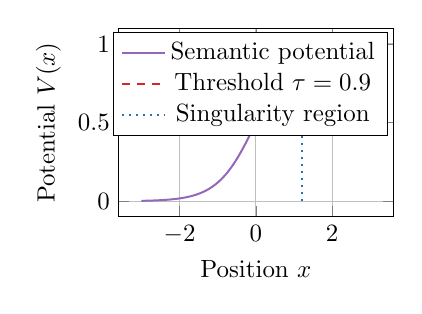
\begin{tikzpicture}[scale=0.9]
    % Potential well visualization
    \begin{axis}[
        width=0.45\textwidth,
        height=0.35\textwidth,
        xlabel={Position $x$},
        ylabel={Potential $V(x)$},
        grid=major,
        samples=100,
        domain=-3:3,
    ]
\addplot[phypurple, thick] {1 / (1 + exp(-2*x))};
\addlegendentry{Semantic potential}

\addplot[phyred, dashed, thick] coordinates {(-3, 0.9) (3, 0.9)};
\addlegendentry{Threshold $\tau = 0.9$}

\addplot[phyblue, dotted, thick] coordinates {(1.2, 0) (1.2, 1)};
\addlegendentry{Singularity region}
\end{axis}
\end{tikzpicture}
\hfill
\begin{tikzpicture}[scale=0.8]
    % Black hole visualization
    \begin{scope}[x={(0.6cm,0.2cm)},y={(-0.3cm,0.6cm)},z={(0,0.8cm)}]
        % Event horizon
        \draw[phyred, very thick] circle (1);
        \filldraw[phyblack] circle (1);
        
        % Accretion disk
        \draw[phyorange, thick, fill=phyorange!20] 
            (0, 0, 0) ellipse (1.5 and 0.3);
            
        % Trajectories
        \foreach \r in {1.5, 2.0, 2.5} {
            \draw[phyblue!\r*30, thick, ->] 
                plot[smooth,tension=0.3] coordinates {
                    (-\r, 0, 0) (-\r*0.7, \r*0.3, 0) (-\r*0.3, \r*0.5, 0) 
                };
        }
        
        % Label
        \node[phyred, above] at (0, 1.3, 0) {Event Horizon};
    \end{scope}
    
    \node[right] at (5, 0) {\textbf{Semantic Event Horizon}};
    \node[right] at (5, -0.5) {Once inside $V(x) > \tau$,};
    \node[right] at (5, -1) {escape requires massive force};
\end{tikzpicture}
\textbf{Left:} Semantic potential with threshold triggering singularity. \textbf{Right:} Visualization of a semantic ``black hole'' where trajectories are trapped.}
\labelfig:semantic-singularity}
\end{figure}

\subsection{Geodesic Trapping}

When a trajectory enters a high-confidence region, it becomes trapped:

\begin{prop}[Geodesic Trapping]
For $V(x) > \tau$, the effective Christoffel symbols scale by $\Omega(x) \gg 1$, creating a ``gravitational well'' that traps the geodesic.
\end{prop}

This mimics psychological phenomena:
\begin{itemize}
\item \textbf{Belief perseverance}: Once committed to a belief, it's hard to change.
\item \textbf{Categorical perception}: Once categorized, perception is biased.
\end{itemize}

\begin{remarque}[Adaptive Behavior]
The singularity mechanism provides:
\begin{enumerate}
\item \textbf{Stability}: High-confidence states are resistant to noise.
\end{enumerate}
This is useful when the model has confidently identified a concept.
\end{remarque}

\begin{prop}[Escape Mechanism]
To escape a singularity, the model requires:
\begin{enumerate}
\item Large input force $F(u_t)$ to overcome the geometric resistance.
\end{enumerate}
This models the cognitive effort required to change a firmly held belief.
\end{prop}

\begin{figure}[htbp]
centering
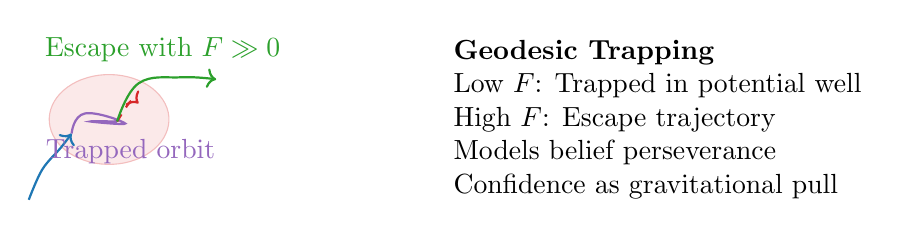
\begin{tikzpicture}[scale=0.85]
    % Trapped trajectory
    \begin{scope}[x={(0.8cm,0.3cm)},y={(-0.4cm,0.6cm)},z={(0,0.8cm)}]
        % Singularity region
        \draw[phyred!30, fill=phyred!10] circle (1);
        
        % Trajectory approaching
        \draw[phyblue, thick, ->] 
            plot[smooth,tension=0.6] coordinates {
                (-2, -1, 0) (-1.5, -0.5, 0) (-1, -0.2, 0) (-0.7, 0, 0)
            };
            
        % Trapped oscillation
        \draw[phypurple, thick] 
            plot[smooth,tension=0.8] coordinates {
                (-0.7, 0, 0) (-0.3, 0.3, 0) (0.2, -0.2, 0) (-0.3, 0.1, 0) (0.1, -0.1, 0)
            };
            
        % Escape attempt (failed)
        \draw[phyred, dashed, thick, ->] 
            plot[smooth,tension=0.5] coordinates {
                (0.1, -0.1, 0) (0.5, 0.2, 0) (0.6, 0.1, 0)
            };
            
        % Escape with large force
        \draw[phygreen, thick, ->] 
            plot[smooth,tension=0.7] coordinates {
                (0.1, -0.1, 0) (0.8, 0.5, 0) (1.5, 0.3, 0) (2, 0, 0)
            };
            
        \node[phypurple] at (0, -0.8, 0) {Trapped orbit};
        \node[phygreen] at (1.5, 1, 0) {Escape with $F \gg 0$};
    \end{scope}
    
    % Explanation
    \node[right] at (5, 1) {\textbf{Geodesic Trapping}};
    \node[right] at (5, 0.5) {Low $F$: Trapped in potential well};
    \node[right] at (5, 0) {High $F$: Escape trajectory};
    \node[right] at (5, -0.5) {Models belief perseverance};
    \node[right] at (5, -1) {Confidence as gravitational pull};
\end{tikzpicture}
caption{Geodesic trapping in a semantic singularity. Trajectories with small input force are trapped in the potential well. Only sufficiently large forces can escape, modeling the cognitive difficulty of changing firmly held beliefs.}
\labelfig:geodesic-trapping}
\end{figure}

\section{Physical Analogies: Relativistic Mass and Viscosity}

The framework connects to fundamental physical concepts.

\subsection{Relativistic Semantic Mass}

The velocity-curvature coupling is analogous to relativistic mass:

\begin{prop}[Relativistic Analogy]
In special relativity:
\[
m_{\text{rel}} = \frac{m_0}{\sqrt{1 - v^2/c^2}}.
\]
In our framework:
\[
\Phi \propto \tanh(K) \quad \text{where} \quad K \propto v^2.
\]
\end{prop}

\begin{remarque}[Geometric Gradient Clipping]
As velocity increases, the effective mass increases, requiring more force to change direction. This is a continuous, differentiable alternative to gradient clipping.
\end{remarque}

\begin{prop}[Intrinsic Stabilization]
The reactive mechanism provides:
\begin{enumerate}
\item \textbf{Geometric gradient clipping}: Large velocities encounter large curvature, naturally limiting acceleration.
\end{enumerate}
Unlike artificial clipping, this is smooth and continuous.
\end{prop}

\begin{figure}[htbp]
centering
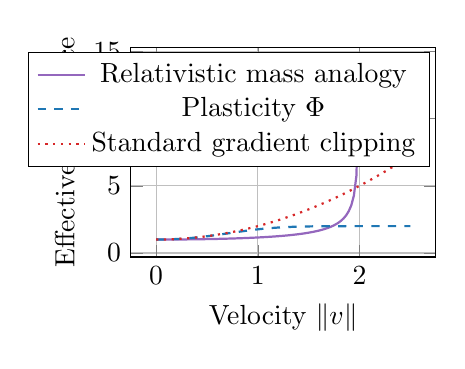
\begin{tikzpicture}
\begin{axis}[
    width=0.45\textwidth,
    height=0.35\textwidth,
    xlabel={Velocity $\|v\|$},
    ylabel={Effective resistance},
    grid=major,
    samples=100,
    domain=0:2.5,
]
\addplot[phypurple, thick] {1 / sqrt(1 - x*x/4)};
\addlegendentry{Relativistic mass analogy}

\addplot[phyblue, dashed, thick] {1 + tanh(x*x)};
\addlegendentry{Plasticity $\Phi$}

\addplot[phyred, dotted, thick] {1 + x*x};
\addlegendentry{Standard gradient clipping}
\end{axis}
\end{tikzpicture}
\hfill
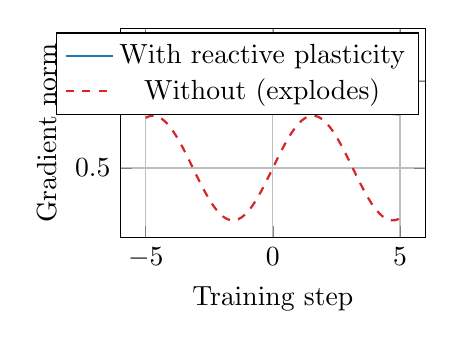
\begin{tikzpicture}
\begin{axis}[
    width=0.45\textwidth,
    height=0.35\textwidth,
    xlabel={Training step},
    ylabel={Gradient norm},
    grid=major,
    samples=100,
]
\addplot[phyblue, thick] {exp(-0.02*x) + 0.1*sin(deg(x))};
\addlegendentry{With reactive plasticity}

\addplot[phyred, dashed, thick] {0.5 + 0.3*sin(deg(x))};
\addlegendentry{Without (explodes)}
\end{axis}
\end{tikzpicture}
\textbf{Left:} Effective resistance comparison. \textbf{Gradient evolution showing intrinsic stabilization from reactive plasticity.}
\labelfig:relativistic-comparison}
\end{figure}

This provides a principled alternative to ad-hoc gradient clipping.

\subsection{Non-Newtonian Semantic Fluids}

The latent space behaves like a non-Newtonian fluid:

\begin{prop}[Fluid Analogy]
\begin{center}
\begin{tabular}{p{0.35\textwidth}p{0.45\textwidth}}
\toprule
Physical Fluid & Semantic Manifold \\ \midrule
Low shear stress & Low velocity (confident) \\
Shear-thickening & High $\Phi$ (confused) \\
Viscosity increase & Curvature increase \\
Low resistance path & Easy semantic transition \\ \bottomrule
\end{tabular}
\end{center}
\end{prop}

\begin{remarque}[Adaptive Behavior]
The manifold is:
\begin{itemize}
\item \textbf{Fluid} during normal reasoning: Low resistance.
\item \textbf{Stiff} during turbulence: High resistance to chaotic motion.
\end{itemize}
\end{remarque}

This ensures the model remains ``fluid'' during normal reasoning but ``stiffens'' when faced with noise or contradictions.

\begin{prop}[Stabilization Mechanism]
Under high-velocity conditions:
\[
\Gamma_{\text{eff}} \cdot v \propto (1 + \Phi) \cdot \Gamma_{\text{static}} \cdot v.
\]
The increased curvature provides geometric damping without explicit regularization.
\end{prop}

\begin{figure}[htbp]
centering
\begin{tikzpicture}[scale=0.9]
    % Viscosity comparison
    \begin{scope}[shift={(0, 0)}]
        \draw[->, thick] (0, 0) -- (5, 0) node[right] {Shear rate (velocity)};
        \draw[->, thick] (0, 0) -- (0, 3) node[above] {Viscosity (resistance)};
        
        % Newtonian
        \draw[phyblue, thick] coordinates {(0, 1) (5, 1)};
        \node[phyblue, above] at (2.5, 1.2) {Newtonian (constant $\eta$)};
        
        % Shear-thickening (our model)
        \draw[phyred, thick] coordinates {(0, 0.5) (1, 0.5) (3, 2) (5, 2.5)};
        \node[phyred, above] at (3.5, 2.7) {Shear-thickening (reactive)};
        
        % Shear-thinning
        \draw[phygreen, dashed, thick] coordinates {(0, 2) (2, 1) (5, 0.5)};
        \node[phygreen, below] at (2.5, 0.3) {Shear-thinning};
        
        % Annotation
        \draw[<->, thick] (2, 2.2) -- (3, 2.2);
        \node[above] at (2.5, 2.4) {Reactive region};
    \end{scope}
    
    % Semantic interpretation
    \begin{scope}[shift={(7, 0)}]
        \node[draw, rectangle, rounded corners, fill=phyblue!20, thick] at (0, 1.5) {Confident: Low resistance};
        \node[draw, rectangle, rounded corners, fill=phypurple!20, thick] at (0, 0) {Uncertain: Moderate resistance};
        \node[draw, rectangle, rounded corners, fill=phyred!20, thick] at (0, -1.5) {Confused: High resistance};
        
        \draw[->, thick] (1.5, 1.5) -- (2.5, 0.75);
        \draw[->, thick] (1.5, 0) -- (2.5, -0.5);
        \draw[->, thick] (1.5, -1.5) -- (2.5, -1.2);
        
        \node[right] at (3, 0) {\textbf{Non-Newtonian}};
        \node[right] at (3, -0.4) {Semantic ``fluid''};
        \node[right] at (3, -0.8) {stiffens under};
        \node[right] at (3, -1.2) {high stress};
    \end{scope}
\end{tikzpicture}
caption{Shear-thickening behavior of the semantic manifold. Unlike Newtonian fluids with constant viscosity, the reactive manifold increases resistance under high-velocity (high-stress) conditions.}
\labelfig:non-newtonian}
\end{figure}

\section{Intrinsic Uncertainty Quantification (UQ)}

Reactive Plasticity provides a deterministic, real-time proxy for uncertainty:

\begin{definition}[Cognitive Temperature]
The cognitive temperature $T$ is the local kinetic energy:
\[
T = \langle v^2 \rangle = \frac{1}{d} \sum_{i=1}^d v_i^2.
\]
\end{definition}

High $T$ indicates the model's inability to reconcile its current state with the input---a direct measure of confusion.

\begin{prop}[Uncertainty Signals]
\begin{enumerate}
\item \textbf{Selective Inference}: Halt computation if $T$ remains too high.
\item \textbf{Safe Autonomy}: Trigger fallback mechanisms when turbulence is detected.
\item \textbf{Active Learning}: Identify data points causing high geometric stress.
\end{enumerate}
\end{prop}

\begin{remarque}[Deterministic UQ]
Unlike Bayesian methods requiring sampling or ensembles, the uncertainty signal is:
\begin{itemize}
\item \textbf{Deterministic}: Single forward pass provides uncertainty.
\item \textbf{Real-time}: Available at every timestep.
\end{itemize}
\end{remarque}

\begin{prop}[Applications]
\begin{center}
\begin{tabular}{p{0.3\textwidth}p{0.5\textwidth}}
\toprule
Application & Mechanism \\ \midrule
Selective inference & Skip computation if $T > T_{\max}$ \\
Safe autonomy & Enter safe mode if $\Phi > \Phi_{\max}$ \\
Active learning & Label $x$ if $T(x) \gg \text{avg}$ \\ \bottomrule
\end{tabular}
\end{center}
\end{prop}

\begin{figure}[htbp]
centering
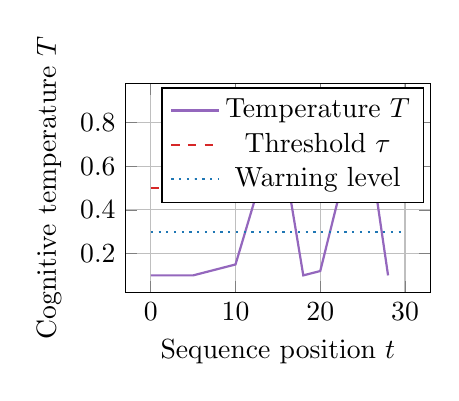
\begin{tikzpicture}
\begin{axis}[
    width=0.45\textwidth,
    height=0.35\textwidth,
    xlabel={Sequence position $t$},
    ylabel={Cognitive temperature $T$},
    grid=major,
    samples=100,
]
\addplot[phypurple, thick] coordinates {
    (0, 0.1) (5, 0.1) (10, 0.15) (15, 0.8) (18, 0.1) (20, 0.12) (25, 0.9) (28, 0.1)
};
\addlegendentry{Temperature $T$}

\addplot[phyred, dashed, thick] coordinates {(0, 0.5) (30, 0.5)};
\addlegendentry{Threshold $\tau$}

\addplot[phyblue, dotted, thick] coordinates {(0, 0.3) (30, 0.3)};
\addlegendentry{Warning level}
\end{axis}
\end{tikzpicture}
\hfill
\begin{tikzpicture}
\begin{axis}[
    width=0.45\textwidth,
    height=0.35\textwidth,
    xlabel={Uncertainty $T$},
    ylabel={Accuracy},
    grid=major,
    samples=100,
]
\addplot[phygreen, thick] {1 - 0.3 * tanh(x)};
\addlegendentry{Accuracy vs. uncertainty}

\addplot[recred, dashed, thick] coordinates {(0.5, 0.85) (0.5, 0.85)};
\node[phyred] at (0.6, 0.9) {Unreliable region};
\end{axis}
\end{tikzpicture}
\textbf{Left:} Cognitive temperature over sequence, showing spikes at ambiguous inputs. \textbf{Right:} Accuracy decreases with uncertainty, validating $T$ as an uncertainty proxy.}
\labelfig:uncertainty-quantification}
\end{figure}

This provides a path toward self-aware neural networks that know when they are confused.

\section{Conclusion}

The Physicality of Confusion demonstrates that the geometric structure of a neural network should be a reactive medium, not a static container:

\begin{prop}[Key Contributions]
\begin{enumerate}
\item \textbf{Finslerian geometry}: Velocity-dependent metrics that model reactive plasticity.
\item \textbf{Semantic singularities}: Extreme confidence creates ``black holes'' that trap trajectories.
\item \textbf{Intrinsic UQ}: Kinetic energy as a deterministic uncertainty proxy.
\end{enumerate}
\end{prop}

\begin{remarque}[Physical Principles]
By transitioning from Riemannian to Finslerian geometry, we allow the model to adapt its internal rigidity to task complexity:
\begin{itemize}
\item \textbf{Certain} regions: Low resistance, fast processing.
\item \textbf{Uncertain} regions: High resistance, careful deliberation.
\end{itemize}
\end{remarque}

This provides a path toward neural networks that possess an intrinsic sense of their own cognitive limits---knowing when to proceed quickly and when to slow down and think carefully.

\clearpage

\appendix

\section{Implementation Code}

\begin{minted}[mathescape, fontsize=\small, frame=lines]{python}
import torch
import torch.nn as nn
import torch.nn.functional as F

class ReactivePlasticity(nn.Module):
    """
    Finslerian manifold with velocity-dependent geometry.
    Implements reactive plasticity and semantic singularities.
    """
    def __init__(self, dim, lambda_plasticity=1.0, tau=0.9, xi=5.0):
        super().__init__()
        self.dim = dim
        self.lambda_plasticity = lambda_plasticity
        self.tau = tau  # Singularity threshold
        self.xi = xi    # Black hole strength
        
        # Static Christoffel symbols (low-rank)
        self.rank = 8
        self.U = nn.Parameter(torch.randn(self.rank, dim) / dim**0.5)
        self.lambda_r = nn.Parameter(torch.randn(self.rank) * 0.1)
        
        # Semantic potential parameters
        self.W_v = nn.Parameter(torch.randn(1, dim) * 0.1)
        self.b_v = nn.Parameter(torch.zeros(1))
        
        # Force projection
        self.W_force = nn.Parameter(torch.randn(dim, dim) * 0.1)
        
    def compute_plasticity(self, v):
        """
        Compute plasticity scalar Phi(x, v).
        Phi = lambda * tanh(mean(v^2))
        """
        kinetic_energy = torch.mean(v ** 2, dim=-1, keepdim=True)
        return self.lambda_plasticity * torch.tanh(kinetic_energy)
    
    def compute_semantic_potential(self, x):
        """
        Compute semantic potential V(x) for singularity detection.
        """
        return torch.sigmoid(torch.mm(x, self.W_v.T) + self.b_v)
    
    def compute_singularity_multiplier(self, x):
        """
        Compute singularity multiplier Omega(x).
        Omega = 1 + sigma(k(V - tau)) * (Xi - 1)
        """
        V = self.compute_semantic_potential(x)
        sharpness = 10.0  # k parameter
        gate = torch.sigmoid(sharpness * (V - self.tau))
        return 1.0 + gate * (self.xi - 1.0)
    
    def compute_christoffel(self, x, v):
        """
        Compute Christoffel symbols via low-rank approximation.
        """
        p = torch.einsum('ij,kj->ik', v, self.U)
        Gamma = torch.einsum('r,ir,jr->ij', self.lambda_r, p, p)
        return torch.tanh(Gamma / 5.0) * 5.0
    
    def compute_effective_christoffel(self, x, v):
        """
        Compute reactive Christoffel symbols with plasticity and singularities.
        Gamma_eff = Gamma_static * (1 + Phi) * Omega
        """
        # Base Christoffel symbols
        Gamma = self.compute_christoffel(x, v)
        
        # Plasticity modulation
        Phi = self.compute_plasticity(v)
        Gamma = Gamma * (1 + Phi)
        
        # Singularity modulation
        Omega = self.compute_singularity_multiplier(x)
        Gamma = Gamma * Omega
        
        return Gamma
    
    def forward(self, x, v, u):
        """
        Forward pass with reactive Finslerian dynamics.
        """
        # Compute force
        F = torch.mm(u, self.W_force.T)
        
        # Compute effective Christoffel symbols
        Gamma = self.compute_effective_christoffel(x, v)
        
        # Geodesic equation: a = F - Gamma(v, v)
        a = F - torch.einsum('ij,j->i', Gamma, v)
        
        # Return acceleration (for integration)
        return a, F
    
    def get_uncertainty(self, v):
        """
        Get cognitive temperature as uncertainty proxy.
        """
        return torch.mean(v ** 2, dim=-1)
    
    def stability_check(self, v, threshold=0.5):
        """
        Check if model is in stable regime.
        Returns True if stable, False if confused.
        """
        uncertainty = self.get_uncertainty(v)
        return uncertainty < threshold


class FinslerianLayer(nn.Module):
    """
    Complete layer with Finslerian dynamics and integration.
    """
    def __init__(self, dim, dt=0.1, **kwargs):
        super().__init__()
        self.dim = dim
        self.dt = dt
        
        self.reactive_plasticity = ReactivePlasticity(dim, **kwargs)
        
    def leapfrog_step(self, x, v, u):
        """
        Leapfrog integration with reactive Finslerian geometry.
        """
        # Compute acceleration at current position
        a, F = self.reactive_plasticity(x, v, u)
        
        # Kick (half step)
        v_half = v + 0.5 * self.dt * a
        
        # Drift (full step with wrapping)
        x_new = (x + self.dt * v_half) % (2 * torch.pi)
        
        # Compute acceleration at new position
        a_new, _ = self.reactive_plasticity(x_new, v_half, u)
        
        # Kick (remaining half step)
        v_new = v_half + 0.5 * self.dt * a_new
        
        return x_new, v_new
    
    def forward(self, x, v, sequence):
        """
        Process sequence with Finslerian dynamics.
        """
        uncertainties = []
        
        for t in range(sequence.shape[0]):
            x, v = self.leapfrog_step(x, v, sequence[t])
            uncertainties.append(self.reactive_plasticity.get_uncertainty(v))
        
        return x, v, torch.stack(uncertainties)
\end{minted}

\section{Connections to Physics}

\begin{prop}[Physical Theory Connections]
\begin{center}
\begin{tabular}{p{0.3\textwidth}p{0.35\textwidth}p{0.35\textwidth}}
\toprule
Our Framework & Classical Physics & Quantum Physics \\ \midrule
Reactive plasticity & Non-Newtonian fluids & Quantum friction \\
Semantic singularities & Black holes & Quantum phase transitions \\
Cognitive temperature & Thermal energy & Zero-point energy \\
Geometric braking & Viscosity & Decoherence \\ \bottomrule
\end{tabular}
\end{center}
\end{prop}

These connections suggest deep links between neural computation and fundamental physics, providing a rich framework for future development.

\end{document}
